\documentclass[pdftex, xcolor=pdftex, dvipsnames, handout, 11pt,t]{beamer}

\definecolor{ThisThemeColour}{HTML}{aa2200}
\definecolor{ThisThemeBg}{HTML}{eeeeee}

\usepackage{../../beamerthemeCS319colour}
\usepackage{multicol}
\usepackage{algorithmicx}

\input{../../CS319stuff.tex}


\newcommand{\colourset}{\lstset{language=C++, 
  basicstyle=\ttfamily\footnotesize,
  keywordstyle=\color{blue}\ttfamily\footnotesize,
  commentstyle=\color{gray}\ttfamily\footnotesize,
  frame=single,numbers=left,
  numberstyle=\footnotesize, stepnumber=2,
  backgroundcolor=\color{BG},
  showstringspaces=false}}

\newcommand{\sset}[1]{\lstset{language=C++,
    showstringspaces=false, 
    basicstyle=\ttfamily\scriptsize,
    keywordstyle=\color{blue}\ttfamily\scriptsize,
    commentstyle=\color{gray}\ttfamily\scriptsize,
    frame=single,
    backgroundcolor=\color{BG},
    texcl=true,
    linewidth=#1\textwidth,
    numbers=left,
    numberstyle=\footnotesize,  stepnumber=2,
    numbersep=5pt,
    numberblanklines=false}%
}




\subtitle{CS319: Scientific Computing (with C++)}
\title{Extra: Reading CSV Files}

\author{Niall Madden}

\date{Week 12: \underline{Extra} (These notes were not covered in class)}

\begin{document}


\frame{


%\column[c]{6cm}
\begin{block}{}
\begin{center}
{\normalsize  \insertsubtitle}\\[1pt]
%{\scriptsize  \insertauthor}


\vspace{.2cm}

\begin{Large}
\textbf{\inserttitle}
\end{Large}


\vspace{.2cm}

{\insertdate}
\end{center}
\end{block}


\begin{center}
  \tableofcontents
\end{center}

}


\setlength{\parskip}{0.2cm}


\RedSet{.8}
\section{Files (recap)}
\vf{

  In Week 9 we learned how to read and write files.
  IN this ``extra'' example, we'll read and write files so-called
  ``CSV files'' that store data for matrices.

  First, we'll recap over some basics...

  \begin{itemize}
    \item To work with files, we need to include the \code{fstream}
      header at the start of our C++ programe.
      \begin{lstlisting}
        #include <cstdlib>
      \end{lstlisting}

    \item To \Emph{read} data from a file, we declare an object of
      type \code{ifstream}.
      \begin{lstlisting}
        ifstream InputFile;
      \end{lstlisting}

    \item To \Emph{write} to a file, declare an object of
      type \code{ofstream}.
      \begin{lstlisting}
        ofstream OutputFile;
      \end{lstlisting}
\end{itemize}

}


\frame[containsverbatim,allowframebreaks]{
  \begin{itemize}
  \item The \code{InputFile} and \code{OutputFile} objects do not get
    have any \emph{actual} files associated with them. To link them to
    files, use the \code{open method}
      \begin{lstlisting}
        InputFile.open("Source.txt");
        OutFile.open("Output.txt");
      \end{lstlisting}
      

    \item \Bf{reading} from a file can be tricky, since we may not
      know how data is stored in it. Often, it is easiest to read a
      single character at a time.
      \begin{lstlisting}
        char c;
        InFile.get( c );
      \end{lstlisting}

    \item \Rf{writing} to a file is easier: we just use the \verb$<<$
      operator, like we do with \code{std::cout}


      \item When finished with a file, we should call the
        \code{close()}method.           


    \item When reading, we also have to check when we get to the
      \code{end} of a file. If there are no more \code{char}acters
      left in the input stream, then the 
      \code{eof()} method evaluates as \icode{true}.

    \item If you have read the contents of a file, and want to go back
      to the start, do this:
      \begin{lstlisting}      
  InFile.clear(); // Clear the eof flag
  InFile.seekg(ios::beg); // rewind to begining.
\end{lstlisting}
\end{itemize}

}


\section{CSV files}
\frame{

As an example of working with files, we'll write a program that
reads data from a  ``\icode{C}omma
\code{S}eparated \icode{V}alues'' (\Emph{\code{CSV}}) file.

There are many accountancy and spread-sheet packages available. It is
necessary for them to be able to share data. Therefore, even though
they all have their own file format, they must be able to read
and write a neutral data type. This is often \icode{CSV}.

Your favourite data-handling system
(e.g., Excel, LibreOffice,...) can read and write these files.

In a \code{CSV} file, the contents of cells from the same row are simply
separated by commas. (Unlike, say, excel files, it does not contain
addition information, such as font type, text
alignment, formulae, etc.

}

\section{Example 1: Library}
\frame{
The first  example we'll look at is based on some  data stored in a
file called \code{Library.csv}:
\begin{figure}[htb]
\centering
   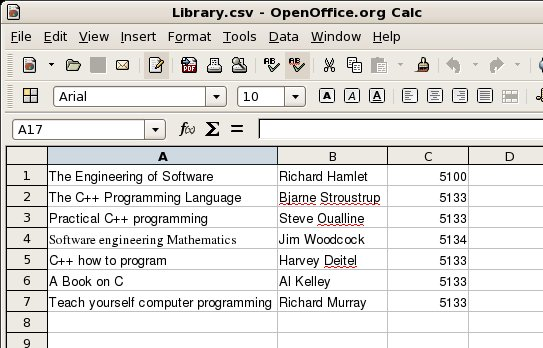
\includegraphics[width=9cm]{Library}
\end{figure}

}


\vf{

When this is saved to a  \code{CSV}  file  we
get
\begin{block}{}
\begin{small}
\begin{verbatim}
The Engineering of Software,Richard Hamlet,5100
The C++ Programming Language,Bjarne Stroustrup,5133
Practical C++ programming,Steve Oualline,5133
Software engineering Mathematics,Jim Woodcock,5134
C++ how to program,Harvey Deitel,5133
A Book on C,Al Kelley,5133
Teach yourself computer programming,Richard Murray,5133
\end{verbatim}
\end{small}
\end{block}
We'll  look at how to  write a C++  program that 
can open this file and read data from it.



We shall assume that we know the structure of the file. In particular,
we'll assume we know how many  columns there are, and what they
contain.
}

\cnset{.9}
\vf{

We'll start by including the necessary headers, including \code{fstream}

\lstinputlisting[linerange=5-10,firstnumber=5,
title={\texttt{00Library-CSV.cpp}}]{00Library-CSV.cpp}
  
}
\lstset{firstnumber=last}
\RedSet{.98}

\vf{

  In the start of the \code{main()} function, we'll define the input
  stream, which we'll call \code{InFile}. We then open the file, and
  verify that no error occurred.
  
\lstinputlisting[linerange=10-21,
title={\texttt{00Library-CSV.cpp} (continued)}]{00Library-CSV.cpp}

}

\vf{
  Then we count the number of lines in the CSV file. The result will
  be used for some dynamic memory allocation.\\
  Once we've read the file, we clear the \code{eof} (end-of-file)
  flag, and set the file pointer back to the \code{beg}inning of the
  file.
  
\lstinputlisting[linerange=22-36,
title={\texttt{00Library-CSV.cpp} (continued)}]{00Library-CSV.cpp}

}

\vf{
  Now that we know the number of lines, we'll declare some arrays for
  storing the data in the file. 
  
  \begin{itemize}
  \item book title (we'll store as a \code{std::string})
  \item Author (also a \code{std::string})
  \item Call number (which we'll treat as an int)
  \end{itemize}
  We reserve memory for each array using the \code{new} operator.
  
\lstinputlisting[linerange=37-40,
title={\texttt{00Library-CSV.cpp} (continued)}]{00Library-CSV.cpp}

}

\vf{
We'll now read the data from the file. First we declare a \code{char}
array of length 100, where we'll store each cell, temporarily.
  We'll read each cell using the \code{get()} method. Note that the
  third argument,  which tells \code{get()} where to stop reading. For
  the first two lines that a comma; for the last it is a new-line. \\
  Then we \code{ignore()} that character.

\lstinputlisting[linerange=41-55]{00Library-CSV.cpp}

}


\vf{
We'll check if it worked by outputting a subset of the
data. Specifically, we'll output the author and title for any book
that has a \code{5133} call number.

\lstinputlisting[linerange=56-64]{00Library-CSV.cpp}

}

\lstset{firstnumber=auto}
\section{Example 2: CSV to Matrix}
\vf{
  In this example, we'll write a program which can read and write
  a \code{Matrix} to/from a file.

  The matrix we'll work with is
  \[
    \begin{pmatrix}
      11.0 & 2.2 & 3.123\\
      -4.2 &  15.6 &   6.0\\
      -7.3 &  -8.0 &  19.0
    \end{pmatrix}
  \]
  The data are stored in the \code{matrix1.cpp} file.
  Here is its contents:
  \cnset{.4}
  \lstinputlisting{matrix1.csv}
  
Once loaded from the file, we'll compute the transpose of this matrix,
and save that to another file.
  
}

\vf{
  To run the following example, you'll need the following files
  \begin{itemize}
  \item \texttt{01Matrix-CSV.cpp} (contains the \code{main()} function)
  \item \texttt{Matrix11.h} and \texttt{Matrix11.cpp} (the latter has
    a minor bug fix).
  \item \texttt{Vector10.h} and \texttt{Vector10.cpp}
  \item \texttt{matrix1.csv}
  \end{itemize}

  Your project must include all three \code{.cpp} files; the \code{.h}
  and \code{.csv} files must be in the appropriate folder.
  You can get the code from
  \url{https://www.niallmadden.ie/2324-CS319/Week12/extras}

  You can also run this code online at
  \code{https://www.online-cpp.com/lRbNcHXsEM}
}

\RedSet{1}
\vf{
  The main program, \code{01Matrix-CSV.cpp} starts with comments and
  the usual include lines (not show here).

  It then includes the headers for the \code{Matrix} and \code{Vector}
  classes.\\ After that, we give the headers for functions that read and
  write the matrices to/from a CSV file.\\
  \code{ReadMatrixCSV()} takes a file name as input and returns a
  \code{Matrix}.\\
  \code{WriteMatrixCSV()} takes as inputs a \code{Matrix}, and string
  containing a file name, and the precision (i.e., number of digits)
  for doubles in the file.
  
\lstinputlisting[linerange=16-21,firstnumber=16,
title={\texttt{01Matrix-CSV.cpp}}]{01Matrix-CSV.cpp}
}

\subsection{\texttt{main()}}  
\vf{
  At the start of the \code{main()} we define a \code{Matrix} object,
  \code{M}, and read its values from a file. The code for the
  \code{ReadMatrixCSV()} function is described further on.
    
\lstinputlisting[linerange=23-30,firstnumber=23,
title={\texttt{01Matrix-CSV.cpp}: main()}]{01Matrix-CSV.cpp}

  }


\vf{
  Next we'll compute the transpose of \code{M}, and write that to a
  file called \code{transpose.m}
    
\lstinputlisting[linerange=31-45,firstnumber=31,
title={\texttt{01Matrix-CSV.cpp}: main()}]{01Matrix-CSV.cpp}

}


\subsection{\texttt{ReadMatrixCSV()}}
\vf{
The function \code{ReadMatrixCSV()} takes a file name, which is
stored as a \code{string}, and tries to open it in a \Emph{input stream}. 

\lstinputlisting[linerange=46-60,firstnumber=46,
title={\texttt{01Matrix-CSV.cpp}: ReadMatrixCSV()}]{01Matrix-CSV.cpp}

}


\vf{
Next the function needs to determine the size of the matrix stored in
the file. We'll be quite lazy about that: we read the first line, and
count the number of commas.\\
We then define a matrix of size $N$, and set its entries to zero.
\lstinputlisting[linerange=62-76,firstnumber=62,
title={\texttt{01Matrix-CSV.cpp}: ReadMatrixCSV()}]{01Matrix-CSV.cpp}
}

\vf{
  Then, after resetting the file pointer to the start of the file,
  we read the contents, alternating between extracting a \code{double}
  (which will be the matrix entries) and a \code{char} which will be
  the comma or new-line.

\lstinputlisting[linerange=78-92,firstnumber=78,
title={\texttt{01Matrix-CSV.cpp}: ReadMatrixCSV()}]{01Matrix-CSV.cpp}
}

\vf{
  When we are finished reading the file contents, we close the file,
  and return the \code{Matrix} object.

\lstinputlisting[linerange=95-97,firstnumber=95,
title={\texttt{01Matrix-CSV.cpp}: ReadMatrixCSV()}]{01Matrix-CSV.cpp}
}


\subsection{\texttt{WriteMatrixCSV()}}    
\vf{
  Our function to write a matrix to a file takes three arguments:
  \begin{enumerate}
    \item The \code{Matrix} object that we are going to write to the
      file;
    \item The name of the file, stored as \code{string} object.
    \item An \code{int} storing the maximum precision we'll use for
      the data. Its default value, set in the header, is 5.
    \end{enumerate}

    We use the stream insertion operator (\code{<<}) for writing the
    data.
    When finished, we close the file.

    The entire code for the function is shown on the next slide.
  }

  \vf{
    \lstinputlisting[linerange=101-121,firstnumber=101,
title={\texttt{01Matrix-CSV.cpp}: WriteMatrixCSV()}]{01Matrix-CSV.cpp}
}

  

\end{document}
